\section{Task 1: Apoapsis Dwell Orbit in Inertial Space}
\label{sec:task1}

\begin{newpar}
USSPACECOM has specified an orbit with the following parameters:
\begin{equation}
T = \SI{24}{\hour}, \qquad e = 0.25, \qquad i = 63.4^\circ, \qquad \omega = \{90^\circ, 270^\circ\}, \qquad 0 \le \Omega \le 180^\circ,
\label{eq:t1-given}
\end{equation}
and with the spacecraft at periapsis at the epoch $t=t_0=0$. We can calculate the semi-major axis from the given period,
\begin{equation}
T = 2\pi\sqrt{\frac{a^3}{\mu}} \;\;\Longrightarrow\;\; a = \left(\frac{\mu T^2}{4\pi^2}\right)^{1/3},
\end{equation}
which we can use for $p = a(1-e^2)$, $r_p = p/(1+e)$, and $r_a = p/(1-e)$:
\end{newpar}

\begin{table}[H]
\centering
\caption{\newtxt{Fixed orbit design parameters, $\mu = \SI{398600}{\kilo\meter\cubed\per\second\squared}$.}}
\label{tab:t1-design}
\color{newtext}
\begin{tabular}{@{}lr@{\qquad}lr@{}}
\toprule
Quantity & Value & Quantity & Value \\
\midrule
$a$ [\si{\kilo\meter}] & $42241.0801$ & $p$ [\si{\kilo\meter}] & $39601.0126$ \\
$e$ [--] & $0.2500$ & $r_p$ [\si{\kilo\meter}] & $31680.8101$ \\
$i$ [\si{\degree}] & $63.4000$ & $r_a$ [\si{\kilo\meter}] & $52801.3501$ \\
$T$ [\si{\hour}] & $24.0000$ & $\Delta t$ [\si{\minute}] & $5$ \\
\bottomrule
\end{tabular}
\end{table}

\subsection*{Task 1-1: Kepler solver}

For an elliptic orbit ($0 \le e < 1$), the \newtxt{true anomaly} at an arbitrary time $t$ \newtxt{is} obtained from \newtxt{$\nu_0$}, $t_0$, $t$, and $\mu$ using the method of Section 3.5\newtxt{~\cite{course-notes}}:
\begin{enumerate}
    \item Solve for $E_0$ from $\nu_0$ using
    \begin{equation}
        E_0 = 2\tan^{-1}\!\left[\sqrt{1-e}\sin\!\left(\frac{\nu_0}{2}\right),\ \sqrt{1+e}\cos\!\left(\frac{\nu_0}{2}\right)\right].
        \label{eq:t1-E0}
    \end{equation}
    \item Solve the general form of Kepler's equation for $E(t)$ to obtain C:
    \begin{equation}
        E - e\sin E = \sqrt{\frac{\mu}{a^3}}(t-t_0) - 2\pi k + \big(E_0 - e\sin E_0\big) \equiv C,
        \label{eq:t1-kepler}
    \end{equation}
    using the fixed-point iteration
    \begin{equation}
        E^{(n+1)} = e\sin E^{(n)} + C,
        \label{eq:t1-fpi}
    \end{equation}
    with the suggested initial guess:
    \begin{equation}
        E^{(0)} = M_0 = E_0 - e\sin E_0,
    \end{equation}
    and run for the suggested number of iterations,
    \begin{equation}
        N = 10\left\lceil \frac{1}{1-e} \right\rceil.
    \end{equation}
    The integer $k$ is the number of periapsis crossings between $t_0$ and $t$, obtained from
    \begin{equation}
        k = \left\lfloor \frac{M_0 + \sqrt{\mu/a^3}\,(t-t_0)}{2\pi} \right\rfloor.
        \label{eq:t1-k}
    \end{equation}
    \item Recover the true anomaly at $t$ from the obtained $E$ (in step \newtxt{2}),
    \begin{equation}
        \nu = 2\tan^{-1}\!\left[\sqrt{1+e}\sin\!\left(\frac{E}{2}\right),\ \sqrt{1-e}\cos\!\left(\frac{E}{2}\right)\right].
        \label{eq:t1-nu}
    \end{equation}
\end{enumerate}
\newtxt{\texttt{step\_kepler(t\_prev, nu\_prev, t, a, e, mu)} in \texttt{kepler.py} implements these three steps.}

\subsection*{Task 1-2: True anomaly at a sequence of times}

\newtxt{The} time grid $\vect{t}$ is built and the true anomaly $\vect{N}$ is computed at each time. With $\Delta t = \SI{5}{\minute}$\newtxt{, $t_0 = 0$, $\nu_0 = 0$,} and $t_n = t_0 + \newtxt{T}$,
\begin{equation}
\vect{t} = \begin{bmatrix} t_0 & t_1 & \cdots & t_n \end{bmatrix}^T,\quad t_i = t_{i-1} + \Delta t
\;\;\Longrightarrow\;\;
n + 1 = 289 \text{ points}.
\end{equation}
\texttt{computeNu(t\_arr, \newtxt{nu\_0, a, e,} miu)} sets $\nu_0$ as the first element of $\vect{N}$, and then calls \texttt{\newtxt{step\_kepler}} once per step with $(t_{i-1},\nu_{i-1},t_i)$ to get $\nu_i$ ($i = 1,\dots,n$).

\subsection*{Task 1-3: Position and velocity}

With $\vect{N}$ from \newtxt{Task 1-2} and the orbital elements $(a,e,\Omega,i,\omega)$, the ECI position and inertial velocity are computed at every $\nu_j$. Each pair is first written in the perifocal frame $P$ (\cref{fig:t1-perifocal}), then rotated to the ECI frame $I$.

\begin{figure}[H]
\centering
% Redrawn from Project 2 Handwork p.4 (perifocal frame, r at true anomaly nu).
% Ellipse: a = 2.5, e = 0.6, b = 2, focus at the origin, nu = 60 deg -> r = 1.2308.
\begin{tikzpicture}[>=Latex, scale=1.15, font=\small]
    % orbit
    \draw[thick, hwblue] (-1.5,0) ellipse (2.5 and 2);
    \fill (0,0) circle (1.6pt);
    \node[below left] at (0,0) {$\vect{p}_z$ (out)};
    % perifocal axes
    \draw[->, thick] (0,0) -- (2.0,0) node[right] {$\vect{p}_x$ (to periapsis)};
    \draw[->, thick] (0,0) -- (0,2.4) node[above] {$\vect{p}_y$};
    % position vector and projections
    \coordinate (S) at (0.6154,1.0659);
    \draw[->, very thick, hwred] (0,0) -- (S) node[above right] {$\vect{r}$};
    \draw[dashed, hwpurple] (S) -- (0.6154,0) node[below] {$r\cos\nu$};
    \draw[dashed, hwpurple] (S) -- (0,1.0659) node[left] {$r\sin\nu$};
    \fill[hwred] (S) circle (1.6pt);
    % true anomaly
    \draw[->, hwgreen] (0.55,0) arc (0:60:0.55);
    \node[hwgreen] at (0.75,0.32) {$\nu$};
    % periapsis / apoapsis
    \fill (1,0) circle (1.2pt) node[below right] {$r_p$};
    \fill (-4,0) circle (1.2pt) node[left] {$r_a$};
\end{tikzpicture}

\caption{Perifocal frame $P$ and the position at true anomaly $\nu$.}
\label{fig:t1-perifocal}
\end{figure}

\subsubsection*{Perifocal position and velocity}
With $p = a(1-e^2)$ and the orbit equation,
\begin{equation}
r(\nu) = \frac{p}{1+e\cos\nu},
\qquad
\vect{r}_P = \begin{bmatrix} r\cos\nu \\ r\sin\nu \\ 0 \end{bmatrix},
\qquad
\ivect{v}_P = \sqrt{\frac{\mu}{p}}\begin{bmatrix} -\sin\nu \\ e + \cos\nu \\ 0 \end{bmatrix}
\;\;\text{(eqn.~2.54~\cite{course-notes})}.
\label{eq:t1-perifocal}
\end{equation}

\subsubsection*{Perifocal to ECI}
$P$ is reached from $I$ by a 3-1-3 rotation through $(\Omega, i, \omega)$, so
\begin{equation}
\vect{r} = \mathbf{R}_3(\Omega)\,\mathbf{R}_1(i)\,\mathbf{R}_3(\omega)\,\vect{r}_P,
\qquad
\ivect{v} = \mathbf{R}_3(\Omega)\,\mathbf{R}_1(i)\,\mathbf{R}_3(\omega)\,\ivect{v}_P,
\label{eq:t1-rot}
\end{equation}
with
\begin{equation}
\mathbf{R}_3(\theta) = \begin{bmatrix} \cos\theta & -\sin\theta & 0 \\ \sin\theta & \cos\theta & 0 \\ 0 & 0 & 1 \end{bmatrix},
\qquad
\mathbf{R}_1(\theta) = \begin{bmatrix} 1 & 0 & 0 \\ 0 & \cos\theta & -\sin\theta \\ 0 & \sin\theta & \cos\theta \end{bmatrix}.
\end{equation}

\subsubsection*{\newtxt{Output}}
\texttt{computeRandV(nu\_arr, a, e, O, i, w, miu)} loops over the $n+1$ values of $\vect{N}$ and \newtxt{returns the results as the rows of}:
\begin{equation}
\mathbf{R} = \begin{bmatrix} \vect{r}^T(t_0) \\ \vect{r}^T(t_1) \\ \vdots \\ \vect{r}^T(t_n) \end{bmatrix},
\qquad
\mathbf{V} = \begin{bmatrix} \ivect{v}^T(t_0) \\ \ivect{v}^T(t_1) \\ \vdots \\ \ivect{v}^T(t_n) \end{bmatrix},
\qquad
\mathbf{R},\,\mathbf{V} \in \mathbb{R}^{(n+1)\times 3}.
\end{equation}
\newtxt{This is repeated for each of the ten $(\omega,\Omega)$ pairs, with the same $\vect{N}$.}

\subsection*{Flowchart for Tasks 1 to 3}

\Cref{fig:t1-flow} shows the order in which the functions of Tasks 1 to 3 are called from \texttt{\newtxt{tasks1to3.py}}, with their inputs (left) and outputs (right).

\begin{figure}[H]
\centering
\scalebox{0.68}{% Function flow for main.py.
\begin{tikzpicture}[
    >=Latex, font=\small, node distance=0.5cm,
    term/.style={circle, draw, thick, minimum size=1.0cm, inner sep=1pt, font=\footnotesize},
    proc/.style={rectangle, draw, thick, minimum height=0.75cm, text width=4.4cm, align=center},
    sub/.style={rectangle, draw, thick, dashed, minimum height=0.75cm, text width=2.6cm, align=center},
    io/.style={font=\footnotesize, align=left},
]
    \node[term] (start) {start};
    \node[proc, below=of start] (prop) {\texttt{propagate\_orbit}\\(loop over $\omega,\Omega$)};
    \node[proc, below=of prop] (ecef) {\texttt{eci2ecef}};
    \node[proc, below=of ecef] (ll) {\texttt{ecef2LonLat}};
    \node[proc, below=of ll] (t12) {Tasks 1--2: 3D orbit and groundtrack plots};
    \node[proc, below=of t12] (t3) {Task 3: hemisphere, crossing point, apoapsis $\Omega$};
    \node[term, below=of t3] (end) {end};

    \node[sub, right=2.6cm of prop] (kep) {\texttt{step\_kepler}\\(incremental)};
    \node[sub, right=2.6cm of ecef] (dcm) {\texttt{dcmI2E}};

    \foreach \a/\b in {start/prop, prop/ecef, ecef/ll, ll/t12, t12/t3, t3/end}
        \draw[->, thick] (\a) -- (\b);
    \draw[<->, thick, hwblue] (prop) -- node[above, io] {$(E_{j-1},\Delta t)$} node[below, io] {$E_j,\nu_j$} (kep);
    \draw[<->, thick, hwblue] (ecef) -- node[above, io] {$(t_j,\Omega_e)$} node[below, io] {$\mathbf{T}_I^E$} (dcm);

    % inputs (left) and outputs (right of the main column)
    \node[io, left=0.3cm of prop] {$a,e,i,\omega,\Omega,T,\Delta t$};
    \node[io, left=0.3cm of ecef] {$\vect{t},\mathbf{R}$};
    \node[io, left=0.3cm of ll] {$\mathbf{R}_e$};
    \node[io, hwred, right=0.3cm of prop] {$\vect{t},\vect{\nu},\mathbf{R},\mathbf{V}$};
    \node[io, hwred, right=0.3cm of ll] {$\vect{\theta}_e,\,\vect{\phi}$};
\end{tikzpicture}
}
\caption{Program flow of \texttt{\newtxt{tasks1to3.py}}.}
\label{fig:t1-flow}
\end{figure}

\subsection*{Task 1-4: Orbits in three dimensions}

The three columns of $\mathbf{R}$ are plotted over an Earth sphere of radius $R_e = \SI{6378.1363}{\kilo\meter}$ (\texttt{earthSphere}, a Python version of \texttt{earthSphere.m} textured with a NASA equirectangular image~\cite{nasa-image}), with line width 2 and \texttt{view(49.5, 22.8)}\newtxt{, one color per value of $\Omega$, and one figure per value of $\omega$ (\cref{fig:t1-orbits})}. The Earth is drawn at $t = 0$, when $ECI$ and $ECEF$ are aligned.

\begin{figure}[H]
\centering
\begin{subfigure}{0.49\textwidth}
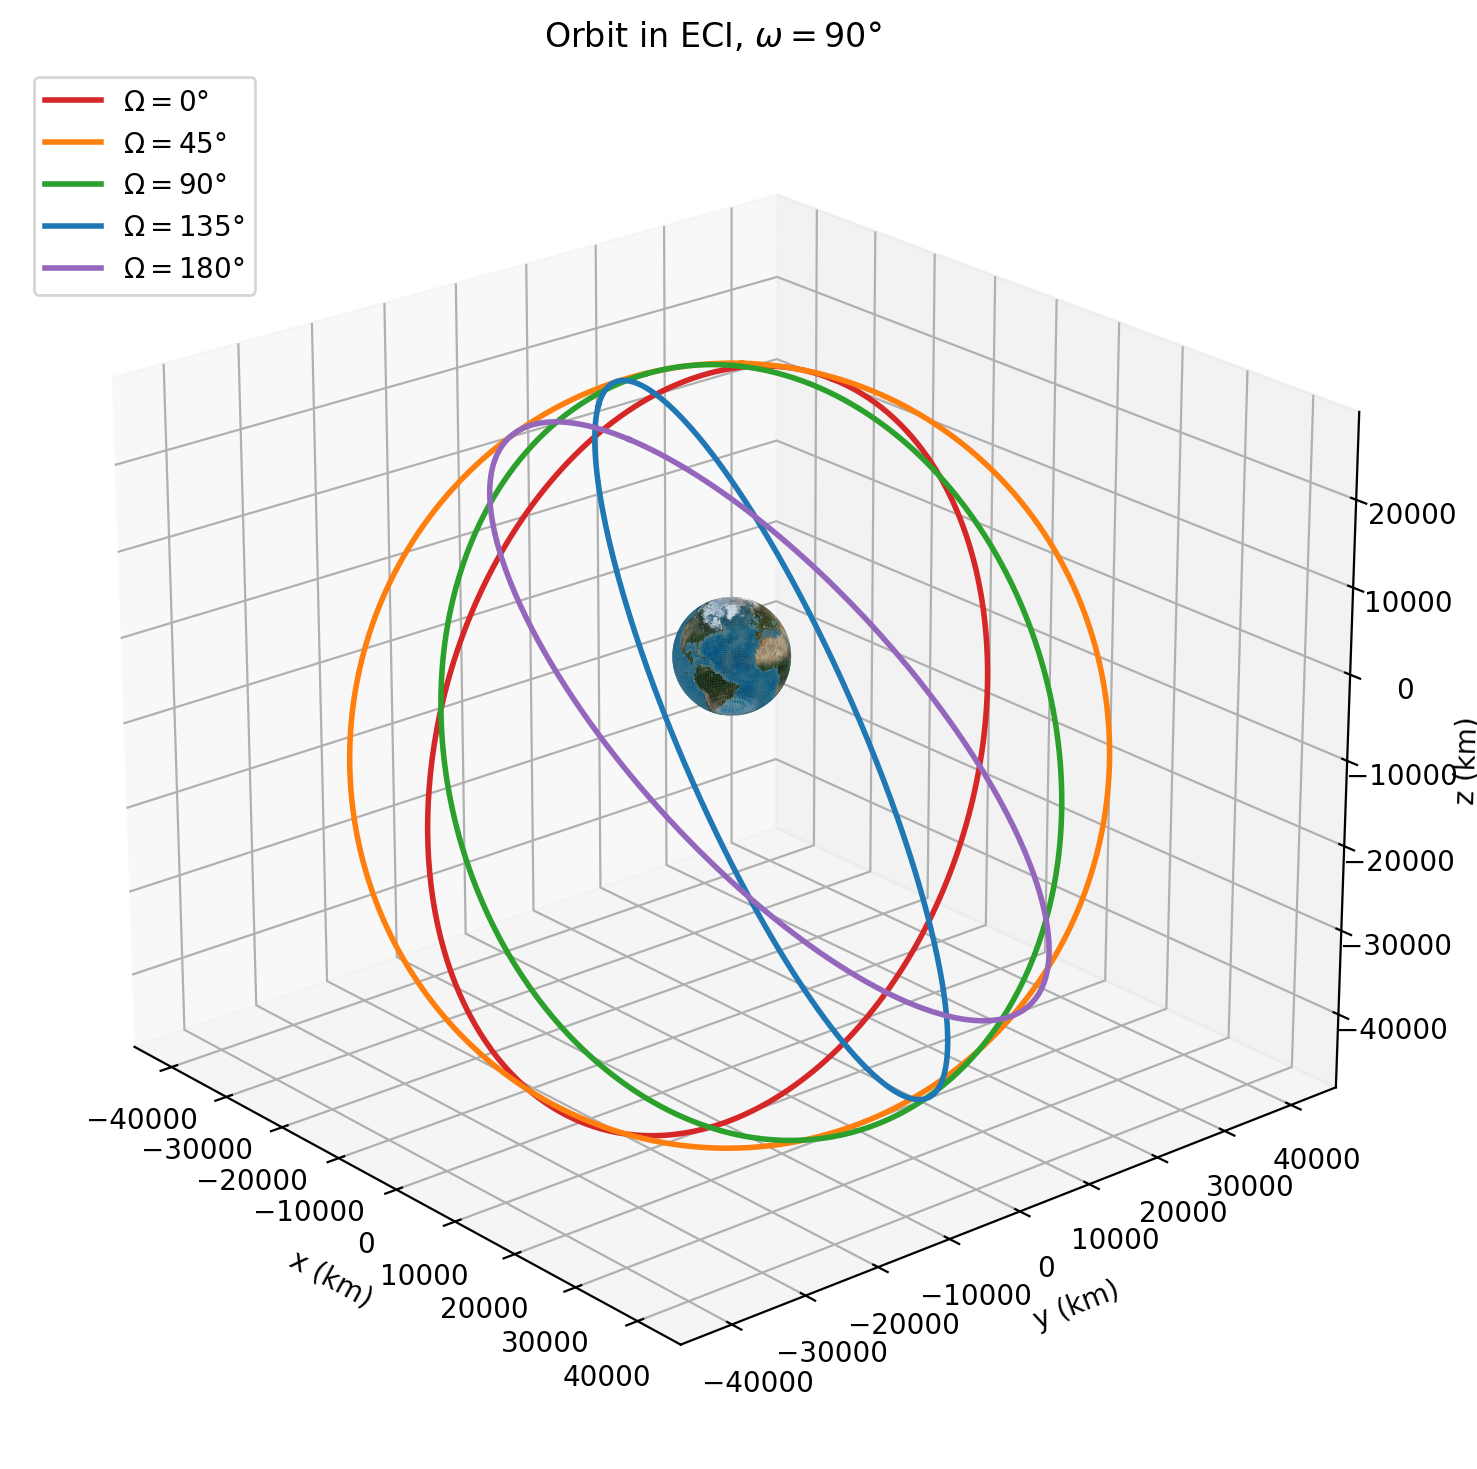
\includegraphics[width=\textwidth]{orbit3d_w90.png}
\caption{\newtxt{$\omega = 90^\circ$}}
\end{subfigure}
\hfill
\begin{subfigure}{0.49\textwidth}
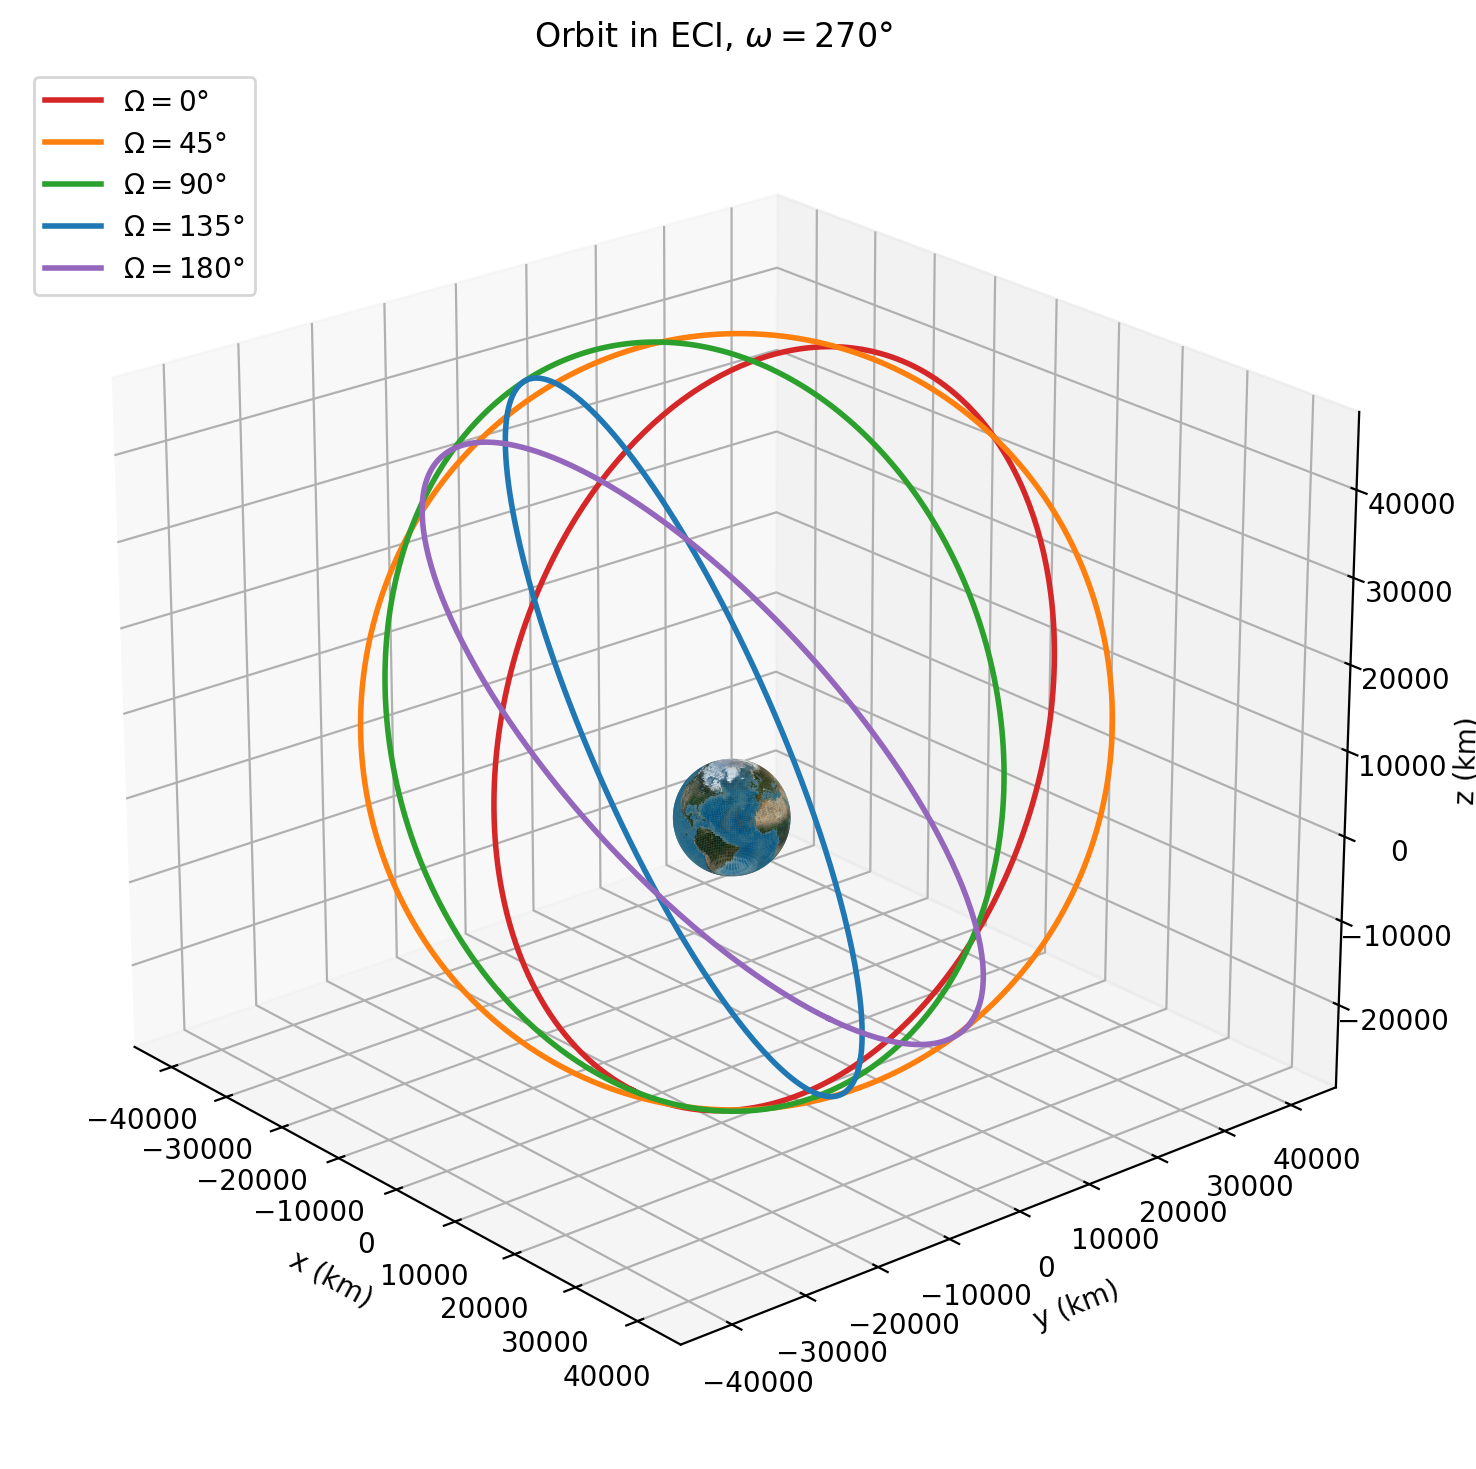
\includegraphics[width=\textwidth]{orbit3d_w270.png}
\caption{\newtxt{$\omega = 270^\circ$}}
\end{subfigure}
\caption{\newtxt{Orbit in the ECI frame over one period for $\Omega = (0,45,90,135,180)^\circ$.}}
\label{fig:t1-orbits}
\end{figure}

\subsubsection*{\newtxt{Structure of the orbit as a function of $\Omega$}}
\newtxt{Changing $\Omega$ rotates the entire orbit 'rigidly' about $\vect{I}_z$. The size, shape, and inclination of the orbit, and the latitudes of periapsis and apoapsis, do not change.}

\subsubsection*{\newtxt{Key difference between $\omega = 90^\circ$ and $\omega = 270^\circ$}}
\newtxt{For $\omega = 90^\circ$,} apoapsis ($\nu = 180^\circ$) lies \newtxt{$\omega + 180^\circ = 270^\circ$} past the ascending node, at the orbit's most \newtxt{southern} point, so the spacecraft is highest and slowest where it is farthest \newtxt{south}. \newtxt{For $\omega = 270^\circ$, apoapsis} lies $90^\circ$ past the ascending node, at the orbit's most northern point, so the spacecraft is highest and slowest where it is farthest north\newtxt{. Each orbit therefore dwells over one hemisphere.}

\FloatBarrier
